\chapter{自然语言到SQL转换方案设计}

\begin{figure}[]
    \centering
    \includegraphics[page=6,width=\linewidth]{figure/figures.pdf}
    \caption{模型整体架构}
    \label{arch}
\end{figure}

在整体架构上,本文使用的是带有注意力机制的编码器-解码器模型,如图\ref{arch}所示。这个框架主要包括了:1. 自然语言与数据库架构编码器,它对自然语言的查询和数据库架构进行协同地编码;2. SQL解码器,它同时考虑自然语言查询,数据库架构和之前交互中的SQL语句,做出决策,逐个标记地生成SQL查询语句。

\section{数据预处理和后处理}

本文在将SQL输入给网络进行训练时先进行了预处理。SQL是人工设计的产物,其具有严格的语法,可以在抽象语法树的层面进行具体的分析和编辑操作。注意到在SQL语句中,由于历史原因,或者是语义准确性的考虑,通常包括了一些繁琐的,抽象程度较低的部分。这些部分将不必要地给SQL的生成带来困难。本文试图将这些繁琐的部分去除,再在SQL生成后确定性地恢复这些内容。

在最终使用的方案中,本文进行了如下的预处理:
\begin{enumerate}
    \item 去除所有JOIN子句中的ON部分。
    \item 去除FROM子句中用于多对多关联的JOIN子句
    \item 在FROM子句中,去除所有在SQL的其他部分引用过的表。若所有表都被去除,则去除整个FROM子句。
\end{enumerate}

在后处理过程中,本文使用以下方法试图恢复这些内容:
\begin{enumerate}
    \item 将所有在SQL中引用过的表添加到FROM子句中。
    \item 根据外键关系,将数据库中的所有表构造成无向图,并使用Kruskal算法求解包含当前FROM子句中的表的最小生成树,根据生成树的边来重建JOIN子句中的ON部分。该步骤也有可能会添加新的表至FROM子句中,例如用于多对多关联的表。构建最小生成树也可能失败,例如数据库架构的外键约束不完整时。若构建失败,则跳过重建JOIN子句ON部分。
\end{enumerate}

\begin{table}[]
    \def\sql#1{\texttt{#1}}
    \def\kw#1{\textcolor{blue}{#1}}
    \def\SELECT{\kw{SELECT }}
    \def\FROM{\kw{FROM }}
    \def\JOIN{\kw{JOIN }}
    \def\AS{\kw{AS }}
    \def\ON{\kw{ON }}

    \begin{tabularx}{\textwidth}{l|X}
    \hline
    自然语言查询 & Who are all the party hosts?…\newline Show the themes of parties they host along with their name.\\ \hline
    原SQL语句 &
    \sql{\SELECT T3.Party\_Theme, T2.Name \FROM party\_host \AS T1 \newline
        \-\hspace{2em} \JOIN host \AS T2 \ON T1.Host\_ID = T2.Host\_ID \newline
        \-\hspace{2em} \JOIN party \AS T3 \ON T1.Party\_ID = T3.Party\_ID} \\ \hline
    预处理后SQL语句 &
    \sql{\SELECT party.Party\_Theme, host.Name} \\ \hline
    \end{tabularx}
    \caption{SQL预处理。party\_host是多对多关联表,host和party表均在SELECT子句中被引用过,所以整个FROM子句全部被去除。}
    \label{preprocess-eg}
\end{table}

表\ref{preprocess-eg}展示了一个预处理的示例。在将SQL输入神经网络前需要将它分割为多个标记。本文使用的分割方法基本思路为将一个关键字、运算符分为一个标记,将对数据库中列或表的引用的表达式视作一个整体,分为一个标记,并与其引用的列或表相关联。有部分关键字总是一同出现,例如GROUP BY等,则将它们视作整体,分为一个标记。在对数据库中列或表的引用的表达式中可能出现多个标识符,别名等。本文对各种情况都手动进行解析,将其关联到它真正引用的表或列。例如表 4 1中的SQL语句最终被分为4个标记。

对于自然语言查询的预处理,本文使用了匹配预训练的预处理方法。例如,当使用XLNet\cite{XLNet19}预训练模型时,使用SentencePiece对语句进行分词,并使用预训练的词嵌入等。

\section{编码器的设计}

编码器的构建是基于大型预训练注意力神经网络,如BERT\cite{bert19}和XLNet\cite{XLNet19}等。本文在之前工作的基础上增加了关系编码机制和上下文编码机制。

\begin{figure}[]
    \centering
    \includegraphics[page=7,width=\linewidth]{figure/figures.pdf}
    \caption{编码器架构}
    \label{enc-arch}
\end{figure}

如图\ref{enc-arch}所示是编码器的整体架构。在输入预训练模型之前,本文在数据库架构部分加入了一些特殊的标记帮助模型分隔各数据库列,并提供额外的上下文信息。预训练模型将为每个输入标记输出一个向量表示,这些特殊标记所对应的输出向量表示将被舍弃。在预训练模型输出的向量表示的基础上,自然语言查询的部分再额外使用一个Bi-LSTM\textsuperscript{E}编码,得到所有单词的最终向量表示$\bm{h}^\mathrm{E}$,将Bi-LSTM\textsuperscript{E}正向和反向的最终隐藏状态拼接,得到整个自然语言查询的向量表示$\bm{c}_t^{turn}$,该向量将作为解码器的初始向量,在后文将详细介绍。对于数据库的列名,分别对每个列名中的多个单词使用Bi-LSTM\textsuperscript{C}编码,并将正向和反向的最终隐藏状态拼接,得到每个列的向量表示$\bm{h}^\mathrm{C}$。

\subsection{上下文编码机制}

上下文编码机制非常简单,但十分高效。它将本轮的自然语言查询和本次交互历史中的查询串联起来,再输入到预训练的编码器中。在之前的工作(如EditSQL\cite{edit19})中,通常使用一个额外LSTM构成的“交互编码器”,以及额外的注意力机制来处理自然言语中的上下文信息。而本文认为,预训练的编码器已经在大规模的语料上进行了无监督训练,其训练预料包含了较长的文本段落。从注意力可视化\cite{attn17}中能够得知,在预训练过程中模型已经能一定程度上掌握理解自然语言上下文的能力,例如理解语言中省略,指代的语义。因此,将上下文信息按照匹配预训练的方法,直接串联起来,输入到预训练编码器中是高效的。

\subsection{关系编码机制}

预训练的编码器最初是为机器翻译等任务而构造的,在设计上它处理的是没有明确结构的自然语言文本信息。而在本任务中我们还需要将高度结构化的数据库架构进行编码。与预训练中包含较长文本段落的预料不同,数据库架构是由表名、列名组成,它们都是短小的词或词组,且不包括完整的语法结构,这可能对编码器编码出高效的数据库架构向量表示造成困难。另外,现有的预训练编码器无法利用数据库架构中的例如主键、外键等关系,缺少这些信息显然将增大该任务的难度。

本文提出的关系编码机制在思想上类似于RAT-SQL\cite{ratsql19}中使用的“关系感知的自注意力” (relation-aware self-attention) 机制,但在具体的做法上有所差异。特别地,本文将该机制融合到了预训练的编码器中。以XLNet为例,下面介绍该机制的具体做法:

关系编码发生在编码器的自注意力层。在通常的理解中,每个自注意力头编码了一种学习到的关系,关系的强度被编码在注意力权重$\alpha_{i,j}^{\left(h\right)}$中。XLNet中的自注意力层使用了“相对位置嵌入”(relative positional embedding) 机制,用以代替最初Transformer中提出的位置嵌入。该机制将公式\ref{attn-forward:1}和\ref{attn-forward:2}替换为:
\begin{equation}
    \alpha_{i,j}^{(h)}=
        \left(\bm{W}_Q^{(h)}\bm{x}_i\right)^T\bm{W}_{k,E}^{(h)}\bm{x}_j+
        \left(\bm{W}_Q^{(h)}\bm{x}_i\right)^T\bm{W}_{k,R}^{(h)}\bm{R}_{i-j}+
        \bm{u}^T\bm{W}_{k,E}^{(h)}\bm{x}_j+
        \bm{v}^T\bm{W}_{k,R}^{(h)}\bm{R}_{i-j}
\end{equation}

其中$\bm{W},\bm{u},\bm{v}$是可学习的参数,$\bm{R}_{i-j}$是使用sinusoid计算的相对位置嵌入,不包含可学习的参数。上述公式中的4项可分别理解为
\begin{enumerate*}
    \item 基于内容的寻址;
    \item 内容相关的位置偏好;
    \item 全局的内容相关偏好;
    \item 全局的位置相关偏好。
\end{enumerate*}
这样的设计是为注意力机制提供了有关相对位置信息的线索,这为模型利用各元素间的位置关系提供了可能。类似地,本文提出的关系编码旨在为注意力机制提供有关已经存在的关系的线索,例如数据库架构中的主键、外键等。在训练过程中,模型可以有选择地利用这些线索学习到如何利用已知的关系。为达成此目标,本文在上述4项的基础上再增加两项:
\begin{equation}
    \alpha_{i,j}^{(h)}=\ldots+
        \left(\bm{W}_Q^{(h)}\bm{x}_i\right)^T\bm{W}_{k,R}^{(h)}\bm{T}_{ij}+
        \bm{t}^T\bm{W}_{k,R}^{(h)}\bm{T}_{ij}
\end{equation}

\begin{table}[]
    \begin{tabularx}{\linewidth}{llll}
    \hline
    x类型 & y类型 & 关系类型              & 描述                 \\ \hline
    表   & 表   & self-table        & 同一表名中的多个单词         \\
    列   & 列   & self-column       & 同一列名中的多个单词         \\ \hline
    列   & 表   & primary-key       & 列x是表y的主键           \\
    列   & 表   & column            & 列x属于表y,但不是主键       \\
    表   & 列   & table             & 表x包含列y             \\
    列   & 列   & sibling-column    & 列x与y属于同一张表         \\ \hline
    列   & 列   & one-to-many-FK    & 列x与y间有一对多的外键关系     \\
    列   & 列   & many-to-one-FK    & 列x与y间有多对一的外键关系     \\
    表   & 表   & one-to-many-table & 表x与y间至少有一组一对多的外键关系 \\
    表   & 表   & many-to-one-table & 表x与y间至少有一组多对一的外键关系 \\ \hline
    列   & 表/列 & other-column      & 列x与y无特殊关系          \\
    表   & 表/列 & other-table       & 表x与y无特殊关系          \\ \hline
    任意  & 任意  & none              & 其他不表示列名或表名的标记      \\ \hline
    \end{tabularx}
    \caption{为数据库架构设计的,用于关系编码中的关系描述。任何两个输入的标记间都有且只有一种关系成立。}
    \label{rel-def}
\end{table}

类似地,这两项分别可理解为内容相关的关系偏好,和全局的关系偏好。其中$\bm{T}_{ij}$表示元素$i$与$j$之间的关系的嵌入,它被初始化为0,这样在训练初期不会对预训练模型产生干扰。为充分表示数据库架构之间的关系,本文总共设计了13种不同的关系,如表\ref{rel-def}所示。

在基于BERT的模型中,本文也类似地实现了关系编码机制。

\section{解码器的设计}

本文使用的解码器是EditSQL\cite{edit19}中的解码器的重新实现。这是一个基于LSTM的,带有注意力机制和编辑机制的解码器。它可以结合之前的SQL语句,当前的自然语言查询和数据库架构,逐个标记地以自回归的形式进行解码。

\subsection{SQL语句编辑机制}

如\citet{edit19}中介绍的,在用户和和系统交互的过程中,倾向于询问一系列紧密相关的问题。需要生成的SQL语句通常和上一轮交互中的SQL语句是有很大部分是重叠的。随着交互的不断进行,SQL语句会越来越复杂,其平均长度会越来越长,但也有更多的标记是和之前的query重叠,需要新增的标记数量是比较稳定的。

基于这样的观察结果, [5]在解码器中加入了SQL语句编辑机制。具体实现包括在上下文向量中加入了上一语句的信息,以及在输出层中加入了拷贝开关,并增加了拷贝的标记的输出路径,具体将会在下文介绍。

\subsection{解码器具体实现}

在解码的第k步骤中,将解码得到的SQL语句标记嵌入$\bm{q}_k$和上下文向量$\bm{c}_k$相连作为LSTM的输入:
\begin{equation}
    \bm{h}_{k+1}^\mathrm{D}=\mathrm{LSTM^D}\left(\left[\bm{q}_k;\bm{c}_k\right],\bm{h}_k^\mathrm{D}\right)
\end{equation}

其中$\bm{h}^\mathrm{D}$是解码器LSTM\textsuperscript{D}的隐藏状态,$\bm{h}_0$初始化为编码器的状态$\bm{c}_t^{turn}$,当解码得到的标记是一个SQL关键字的时候,$\bm{q}_k$是一个可学习的关键字的嵌入,当它是一个列名的时候,$\bm{q}_k$则是由编码器输出的,该列的向量表示。

上下文向量$\bm{c}_k$包含了解码器隐藏状态到自然语言、数据库架构中列的向量表示和上一次的SQL语句的注意力。解码器隐藏状态到数据库列的注意力可表示为:
\begin{align}
    \bm{s}_l&=\bm{W}_\mathrm{column-att}\bm{h}_k^\mathrm{D}\cdot\bm{h}_l^\mathrm{C}\\
    \bm{\alpha}^\mathrm{column}&=\softmax\left(\bm{s}\right)\\
    \bm{c}_k^\mathrm{column}&=\sum_{l}{\bm{\alpha}_l^\mathrm{column}\times\bm{h}_l^\mathrm{C}}
\end{align}

其中,$\bm{h}_l^\mathrm{C}$为数据库中第$l$列的向量表示。解码器隐藏状态到自然语言的注意力可表示为:
\begin{align}
    \bm{s}_i&=\bm{W}_\mathrm{utterance-att}\bm{h}_k^\mathrm{D}\cdot\bm{h}_i^\mathrm{E}\\
    \bm{\alpha}^\mathrm{utterance}&=\softmax\left(\bm{s}\right)\\
    \bm{c}_k^\mathrm{utterance}&=\sum_{i}{\bm{\alpha}_i^\mathrm{utterance}\times\bm{h}_i^\mathrm{E}}
\end{align}

其中$\bm{h}_i^\mathrm{E}$为拼接后的当前和历史记录中的自然语言查询中的第i个单词的向量表示。类似地,解码器隐藏状态到上一次的SQL语句的注意力可表示为:
\begin{align}
    \bm{s}_i&=\bm{W}_\mathrm{query-att}\bm{h}_k^\mathrm{D}\cdot\bm{h}_i^\mathrm{Q}\\
    \bm{\alpha}^\mathrm{query}&=\softmax\left(\bm{s}\right)\\
    \bm{c}_k^\mathrm{query}&=\sum_{i}{\bm{\alpha}_i^\mathrm{query}\times\bm{h}_{t-1,i}^\mathrm{Q}}
\end{align}

其中,$\bm{h}_{t-1,i}^\mathrm{Q}$表示上一个SQL语句中的第i个标记的向量表示。这个表示是由另一个LSTM编码得到的,上下文向量是由上述三者连接在一起得到:
\begin{equation}
    \bm{c}_k=\left[\bm{c}_k^\mathrm{column};\bm{c}_k^\mathrm{utterance};\bm{c}_k^\mathrm{query}\right]
\end{equation}

在输出层中,模型通过当前LSTM的隐藏状态$\bm{h}_k^\mathrm{D}$和上下文向量$\bm{c}_k$,做出SQL语句解码的决策,其决策分为三个分支:1. 解码一个SQL关键字 (SELECT, WHERE等);2. 解码一个数据库表或者列;3. 从上一个SQL语句中拷贝一个标记。在跨领域的设定中,每次解码时SQL关键字都是一样的,而数据库架构则不同,所以使用不同的模块来解码两者是非常关键的。在拷贝的分支中,我们预测了一个独立的开关来控制是否需要拷贝。最终,使用softmax来综合各个分支,并获取生成标记的概率分布。
\begin{equation}
    \bm{o}_k=\tanh{\left(\bm{W}_o\left[\bm{h}_k^D;\bm{c}_k\right]\right)}
\end{equation}
拷贝开关预测:
\begin{align}
    p_\mathrm{copy}=\sigma\left(\bm{W}_\mathrm{copy}\bm{o}_k+b_\mathrm{copy}\right)\\
    p_\mathrm{gen}=1-p_\mathrm{copy}
\end{align}
对于拷贝分支概率分布,$\bm{P}_\mathrm{prevSQL}$表示在上一SQL语句中每个标记复制到当前位置的概率:
\begin{align}
    \bm{P}_\mathrm{prevSQL}=\softmax\left(\bm{W}_\mathrm{prevSQL}\bm{o}_k\cdot\bm{h}_{t-1}^Q\right)
\end{align}
对于生成分支概率分布,$\bm{P}_\mathrm{gen}$表示生成任何可能的标记的概率:
\begin{align}
\bm{m}_{SQL}=\bm{W}_{SQL}\bm{o}_k+\bm{b}_{SQL}\\
\bm{m}_{column}=\bm{W}_{column}\bm{o}_k\cdot\bm{h}^C\\
\bm{P}_\mathrm{gen}=softmax\left(\left[\bm{m}_{SQL};\bm{m}_{column}\right]\right)
\end{align}
最终决策的生成下一个标记的概率分布为:
\begin{align}
p\left(y_k^t\right)=p_\mathrm{copy}\sum_{l\in\left\{l|y_l^{t-1}=y_k^t\right\}}{\bm{P}_\mathrm{prevSQL}\left(y_l^{t-1}\right)}+p_\mathrm{gen}\cdot\bm{P}_\mathrm{gen}(y_k^t)
\end{align}
其中,$\bm{P}_\mathrm{gen}(y_k)$表示生成$y_k$标记的概率,$\sum_{l\in\left\{l|y_l^{t-1}=y_k^t\right\}}{\bm{P}_\mathrm{prevSQL}\left(y_l^{t-1}\right)}$表示在上一SQL语句中,所有出现的$y_k$标记的复制概率之和。当一次交互中的首个SQL语句解码时,不存在上一个SQL语句,这时将$p_\mathrm{copy}$设为0并跳过拷贝分支。注意到对于所有可能的$y_k$,$p\left(y_k\right)$之和将仍为1,无需进一步归一化。

\section{本章小结}

本章详细介绍了实现自然语言到SQL转换任务的方案,这是一个端到端的神经网络。其中相对于之前的工作,有以下创新:使用适当的SQL预处理和后处理过程,帮助网络高效的生成准确的SQL语句;加入上下文编码机制,帮助网络更好地理解自然语言上下文;在预训练模型中加入关系编码机制,能将预定义的主键,外键等信息编码,并指导自注意力机制,提升编码质量。
